
%----------------------------------------------------------------------------------------
%	Lecture 3
%----------------------------------------------------------------------------------------

\section*{\centering Derivatives of Products, Quotients, Sine and Cosine}  

\bigbreak
\section{Derivative Formulas}

There are two kinds of derivative formulas:

\begin{enumerate}
\item Specific Examples: $\diff{}{x} x^n$ or $\diff{}{x} \left( \frac{1}{x} \right) $
\item General Examples: $(u+v)' = u' + v'$ and $(cu)' = cu'$ (where $c$ is constant)
\end{enumerate}

A notational convention we will use today is:
$$(u+v)(x) = u(x) + v(x); \quad (uv)(x) = u(x)v(x)$$ 

\subsection{Proof of $(u+v)' = u'+v'$. (General)}

Start by using the definition of derivative.
\begin{equation*}
\begin{split}
	(u+v)'(x)	& = \lim_{\Delta x \to 0} \frac{(u+v)(x+\Delta x) - (u+v)(x)}{\Delta x} \\
				& = \lim_{\Delta x \to 0} \frac{u(x+\Delta x)+v(x+\Delta x) - u(x) - v(x)}{\Delta x} \\
				& = \lim_{\Delta x \to 0} \left\{ \frac{u(x+\Delta x) - u(x)}{\Delta x} + \frac{v(x+\Delta x) - v(x)}{\Delta x} \right\} \\
	(u+v)'(x)	& = u'(x) + v'(x)
\end{split}
\end{equation*}

Follow the same procedure to prove $(cu)' = cu'$.

\subsection{Derivatives of $\sin x$ and $\cos x$. (Specific)}

Last time, we computed.
\begin{equation*}
\begin{split}
	\diff{}{x} (\sin x) |_{\substack{x=0}} & = 
		\lim_{\Delta x \to 0} \frac{\sin(0 + \Delta x) - \sin(0) }{\Delta x} = 
		\lim_{\Delta x \to 0} \frac{\sin(\Delta x)}{\Delta x} = 1 \\
	\diff{}{x} (\cos x) |_{\substack{x=0}} & = 
        \lim_{\Delta x \to 0} \frac{\cos(0 + \Delta x) - \cos(0) }{\Delta x} = 
        \lim_{\Delta x \to 0} \frac{\cos(\Delta x)-1}{\Delta x} = 0 \\
\end{split}
\end{equation*}

So we know the value of $\diff{}{x} \sin x$ and $\diff{}{x} \cos x$ at $x = 0$. Let us find for arbitary $x$. 
$$\diff{}{x} \sin x = \lim_{\Delta x \to 0} \frac{\sin(x+\Delta x) - \sin(x)}{\Delta x}$$

Recall : $$\sin(a+b) = \sin(a)\cos(b) + \cos(a)\sin(b)$$

So,
\begin{equation*}
\begin{split}
	\diff{}{x} \sin x 
		& = \lim_{\Delta x \to 0} \frac{\sin x \cos \Delta x + \cos x \sin \Delta x - \sin x}{\Delta x} \\
		& = \lim_{\Delta x \to 0} \left[ \frac{\sin x (\cos \Delta x - 1)}{\Delta x} \frac{\cos x \sin \Delta x}{\Delta x} \right] \\
		& = \lim_{\Delta x \to 0} \sin x \left( \frac{\cos \Delta x - 1}{\Delta x} \right) + \lim_{\Delta x \to 0} \cos x \left( \frac{\sin \Delta x}{\Delta x} \right)
\end{split}
\end{equation*}

Since $\frac{\cos \Delta x - 1}{\Delta x} \to 0$ and that $\frac{\sin \Delta x}{\Delta x} \to 1$, the above equation simplifies to $$\diff{}{x} \sin x = \cos x$$

A similar calculation gives
$$\diff{}{x} \cos x = - \sin x$$


\subsection{Product formula (General)}

$$(uv)' = u'v+uv'$$

Proof:
$$(uv)' = \lim_{\Delta x \to 0} \frac{(uv)(x+\Delta x) - (uv)(x)}{\Delta x}
		= \lim_{\Delta x \to 0} \frac{u(x+\Delta x)v(x+\Delta x) - u(x)v(x)}{\Delta x}$$

Now obviously, $$u(x+\Delta x)v(x) - u(x+\Delta x)v(x) = 0$$

So adding that to the numerator won't change anyhting.
$$
(uv)' = \lim_{\Delta x \to 0} 
	\frac{
		u(x+\Delta x)v(x)
		- u(x)v(x)
		+ u(x+\Delta x)v(x+\Delta x)
		- u(x+\Delta x)v(x)
	}{\Delta x}
$$

We can re-arrange to get
$$
(uv)' = \lim_{\Delta x \to 0} 
	\left( \frac{u(x+\Delta x) - u(x)}{\Delta x} \right) v(x) +
	u(x+\Delta x) \left( \frac{v(x+\Delta x) - v(x)}{\Delta x} \right) 
$$

Remember, the limit of sum is the sum of limits.
$$
(uv)' = \left[ \lim_{\Delta x \to 0} \frac{u(x+\Delta x) - u(x)}{\Delta x} \right] v(x) +
	\lim_{\Delta x \to 0} \left( u(x+\Delta x) \left[ \frac{v(x+\Delta x) - v(x)}{\Delta x} \right] \right)
$$
$$(uv)'(x) = u'(x)v(x) + u(x)v'(x)$$

Note: we also used the fact that $$ \lim_{\Delta x \to 0} u(x+\Delta x) = u(x) \quad \text{(true because $u$ is continuous)}$$

This proof of product rule implies that both $u$ and $v$ have derivatives, which implies both functions are continuous.

\begin{figure}[h!]
	\centering
	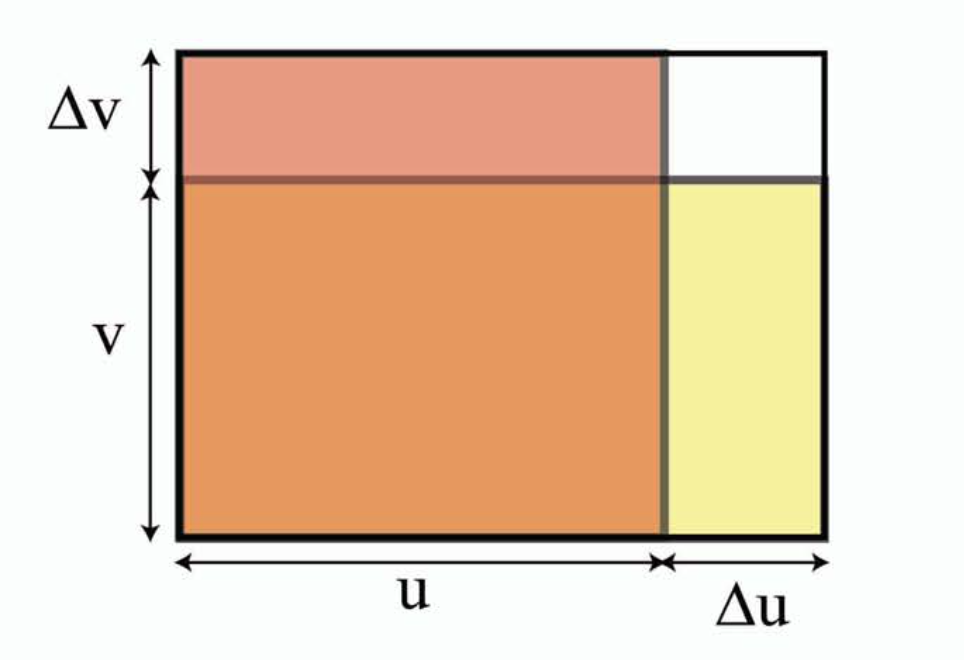
\includegraphics[scale=0.4]{./images/lecture_3_figure_1.png}
	\caption{A graphical ``proof'' of product rule.}    
\end{figure}

\subsubsection*{An intuitive justification:}

Define $\Delta u$, the change in $u$, by $$\Delta u = u(x+\Delta x) - u(x)$$

We want to find out the change in area of the rectangle. As we can see, 

$$\Delta(uv) = (\Delta u)v + u(\Delta v) + (\Delta u)(\Delta v)$$

If $\Delta u$ and $\Delta v$ are small then $(\Delta u)(\Delta v) \approx 0$, so we can ignore this area.
$$\Delta(uv) = (\Delta u)v + u(\Delta v)$$

Dividing by $\Delta x$ and taking the limit, we get
$$(uv)' = u'v + uv'$$

\subsection{Quotient Rule (General)}

To calculate the derivative of $u/v$, we use the notations $\Delta u$ and $\Delta v$ above.
\begin{equation*}
\begin{split}
	\frac{u(x+\Delta x)}{v(x+\Delta x)} - \frac{u(x)}{v(x)}
		& = \frac{u + \Delta u}{v + \Delta v} - \frac{u}{v} \\
		& = \frac{(u+\Delta u)v - u(v+\Delta v)}{v(v+\Delta v)} \\
		& = \frac{(\Delta u)v - u(\Delta v)}{v(v+\Delta v)}
\end{split}
\end{equation*}

Hence,
$$
\frac{1}{\Delta x} \left( \frac{(\Delta u)v - u(\Delta v)}{v(v+\Delta v)} \right)
	= \frac{(\frac{\Delta u}{\Delta x})v - u(\frac{\Delta v}{\Delta x})}{v(v+\Delta v)}
	\to \frac{v\diff{u}{x} - u\diff{v}{x}}{v^2} \text{ as } \Delta x \to 0
$$

Therefore, 
$$(\frac{u}{v})' = \frac{u'v - uv'}{v^2}$$



\subsection{Power Rule : Derivative of $x^n$ where $n = 1,2,3\ldots$ (Specific)}

What is $\diff{}{x} x^n$?

$$ \diff{}{x} x^n = \lim_{\Delta x \to 0} \frac{(x+\Delta x)^n - x^n}{\Delta x} $$

Since, $$ (x+\Delta x)^n = (x+\Delta x)(x+\Delta x)\ldots(x+\Delta x) \text{ ($n$ times) } $$

We can rewrite this as $$ x^n + n(\Delta x)x^{n-1} + O((\Delta x)^2) $$

So, $$ \diff{}{x} x^n = \lim_{\Delta x \to 0} \frac{x^n + n(\Delta x)x^{n-1} + O((\Delta x)^2) - x^n}{\Delta x} = \lim_{\Delta x \to 0} nx^{n-1} + O(\Delta x) $$

Therefore, $$ \boxed{ \diff{}{x} x^n = nx^{n-1} } $$

This result extends to polynomials. For example, $$ \diff{}{x}(x^2+3x^10) = 2x + 30x^9 $$

\subsection{Derivative of $\frac{1}{x}$}
Taking the limit
\begin{equation*}
\begin{split}
	\diff{}{x} \frac{1}{x} 
		& = \lim_{\Delta x \to 0} \frac{1}{\Delta x} \left( \frac{1}{x+\Delta x} - \frac{1}{x} \right) \\
		& = \lim_{\Delta x \to 0} \frac{1}{\Delta x} \left( \frac{x - (x+\Delta x)}{x(x+\Delta x)} \right) \\
		& = \lim_{\Delta x \to 0} \frac{-1}{x(x+\Delta x)} \\
	\diff{}{x} \frac{1}{x} & = \frac{-1}{x^2}
\end{split}
\end{equation*}
